\documentclass[UTF8]{ctexart} % say 
\usepackage{tikz} 
\usetikzlibrary{intersections}

\begin{document}
We are working on 
\begin{tikzpicture}[scale=3]
    %\clip (-0.1,-0.2) rectangle (1.1,0.75);
    \draw[->,very thick] (-2,0) -- +(4,0); 
    \draw[->,very thick] (0,-2) -- +(0,4);
    \draw (0,0) circle[radius=1cm];
    \filldraw[fill=green!20,draw=green!50!black] (0,0) -- (3mm,0mm) 
    arc [start angle=0, end angle=30, radius=3mm] -- cycle;
    \draw[red,very thick] (30:1cm) -- +(0,-0.5);
    \draw[blue,very thick] (30:1cm) ++(0,-0.5) -- (0,0);
    \path [name path=upward line] (1,0) -- (1,1); 
    \path [name path=sloped line] (0,0) -- (30:1.5cm);
     % a bit longer, so that there is an intersection
% (add `\usetikzlibrary{intersections}' after loading tikz in the preamble) 
    \draw [name intersections={of=upward line and sloped line, by=x}]
        [very thick,orange] (1,0) -- (x);
        
    \draw (1,1)--(2,2) [xshift=2pt,yshift=4pt]; 
    \draw (1,1)--(2,2)[yshift=6pt];
    \draw (0.15,0.15) node {原点};
    \foreach \x/\xtext in {-2,-1.5,-1/-\frac{3}{2},1}
        \draw(\x cm,1pt)--(\x cm,0pt) node [anchor=north]{$\xtext$};
\end{tikzpicture}.
second picture
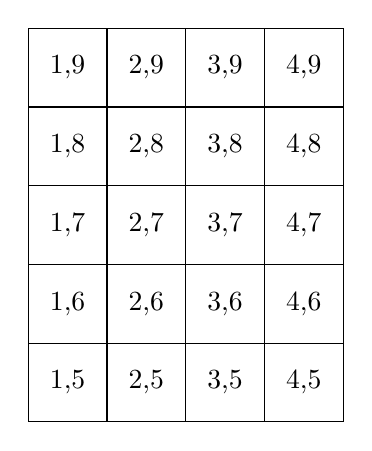
\begin{tikzpicture}
\foreach \x in {1,...,4}
    \foreach \y in {5,...,9}
        {
            \draw (\x,\y)+(-.5,-.5) rectangle ++(.5,.5);
            \draw (\x,\y) node{\x,\y};
         } 
\end{tikzpicture}
\end{document}